% !TeX encoding = UTF-8
% !TeX program = pdflatex
% !TeX spellcheck = en-US

\documentclass[11pt]{article}

\usepackage[english]{babel}
\usepackage{graphicx}
\usepackage{listings}
\usepackage{xcolor}   % for \textcolor
\usepackage{tikz,pgfplots}
\usepackage[htt]{hyphenat}
\usepackage{url}

\lstset
{
  language=C,
  numbers=left,
  stepnumber=1,
  breaklines=true,
  basicstyle=\ttfamily,
  keywordstyle=\color{blue}\ttfamily,
  stringstyle=\color{red}\ttfamily,
  commentstyle=\color{green}\ttfamily,
  morecomment=[l][\color{magenta}]{\#}
  columns=fullflexible,
  postbreak=\mbox{\textcolor{red}{$\hookrightarrow$}\space},
  escapeinside={(*@}{@*)},
}
\lstdefinestyle{nonumbers}
{numbers=none}

\title{Openfibers Kernel Module Description \\ \bigskip \large Advanced Operating Systems -  Sapienza}
\author{Pietro Borrello}
\date{\today}

\begin{document}

\maketitle

\tableofcontents
\newpage

\section{Introduction}
In this paper we are going to present a brief description of a from scratch implemented Linux Kernel Module, which aims to give support to userspace processes to Fibers utilities. A fiber is a unit of execution of a process that must be manually scheduled by the application \cite{fibers}. Each fiber runs in the thread that scheduled it, and any thread of a process can schedule any fibers owned by such process. A fibers that runs in a thread, runs in top of its contexts until that thread manually switches to any other fiber. When a thread running fibers is preempted, its currently running fiber is preempted. The same fiber resumes running when its thread resumes. Each fiber has the possibility to create and manage a Fiber Local Storage, in which it can use transparently a unique copy of a defined variable

\section{APIs}
The system has to offer some APIs to userspace processes, to let them ask the kernel to create and manage fibers.

\begin{itemize}
\item{\textbf{ConvertThreadToFiber}}: creates a fiber in the current thread. The calling thread is now the currently executing fiber.
\item{\textbf{CreateFiber}}: create a new fiber from an existing fiber, being able to specify the stack size, the starting address, and the data the fiber will start from
\item{\textbf{SwitchToFiber}}: execute any fiber created with CreateFiber or switch to a previously running fiber
\item{\textbf{FlsAlloc}, \textbf{FlsFree}, \textbf{FlsGetValue}, \textbf{FlsSetValue}}: to manage the fiber local storage of the current fiber
\end{itemize}

\section{Module Design Goals}
The Fiber support will be served by the Linux Kernel Module exposing a character device in \texttt{/dev/openfibers} to communicate with, in order to be able to ask the kernel for fibers operations from userspace. The module will manage each fiber process context independently to favor isolation between all the processes, so that any process will not compete with the others for fibers resources. Moreover isolating the fibers for each process doesn't increase the attack surface for any user using fibers: with all the fibers in the same structure any bug in the code would allow any process to corrupt sensible structure of any other (i.e. a root process).

The module is expected to work in an SMP system, and to favor the coexistence of multiple processes, and multiple thread, running at the same time, and with multiple fibers active each. Accesses to shared structures should be as quick as possible, possibly avoiding locks.

The module should expose information about active or running fibers to userspace, including the starting function, the number of successful and failed activation, the owner and the time of living. This should be ideally done exposing a {\tt fibers} folder under {\tt /proc/<pid>/fibers} containing a file for each fiber.

\subsection{Fibers Operation}
The first thread to be converted to fibers, should implicit initialize the fiber context for all the successive thread conversion and switches, and should set its current fiber running. After a thread is converted to a fiber, it should be able to create new fibers, setting the starting point and the initial parameters. Whenever a thread switches to a different fiber, we should guarantee it will work, unless the target fiber is yet running. Any concurrent execution of the same fiber should be avoided. We predicted the fiber switch to be the most frequent operation in fiber context, so it is critical to design it to be efficient.

Any fiber switch in principle should be designed to be non blocking, since any delay in the switch, would negatively affect the most part of applications designed on top of fibers. We allow instead the kernel to rely on lock for safe initialization and safe cleanup, as they are expected to be less frequent, but critical to be done in isolation.

\subsection{FLS Operation}
We expect every fiber will have a highly dense usage of {\tt FLS} facilities. Therefore we just keep it simple. Any thread should access the fiber local storage without any delay with respect to normal variable accesses (without accounting for the syscall delay needed to communicate with the kernel). Therefore we refused to accept any design that would introduce a non constant number of memory accesses for local storage operations.

\subsection{Components}
The Fiber implementation will have two components: A loadable linux kernel module that will implement the desired operations, at kernel level, to be as efficient as possible; and a shared library to be included in user-level processes to provide a user friendly interface with the kernel module. To favor information hiding, and to simplify interaction, the library should manage the formats and structures needed by kernel level APIs, exposing to the user a simple directly callable interface.


\section{Module Implementation}
The Linux Kernel Module managing fibers is implemented as a character device in {\tt /dev/openfibers} exposing a single entry point to ask for operations through the {\tt ioctl()} system call. The following commands to be issued to the syscall are declared: they reflect all the possible APIs operations that can be issued to the Fibers.

\begin{lstlisting}
#define OPENFIBERS_IOCTL_CREATE_FIBER [...]
#define OPENFIBERS_IOCTL_SWITCH_TO_FIBER [...]
#define OPENFIBERS_IOCTL_CONVERT_TO_FIBER [...]
#define OPENFIBERS_IOCTL_FLS_ALLOC [...]
#define OPENFIBERS_IOCTL_FLS_FREE [...]
#define OPENFIBERS_IOCTL_FLS_SET [...]
#define OPENFIBERS_IOCTL_FLS_GET [...]
\end{lstlisting}

The module maintains process fiber information in a Red Black Tree \cite{rbtree}. The tree contains the set of fibers for each thread group, indexed by {\tt tgid}. Any {\tt tgid} node is declared as follows:
\begin{lstlisting}
struct fibers_by_tgid_node
{
    struct rb_node node;
    pid_t tgid;
    struct rb_root *fibers_root;
    struct rw_semaphore fibers_root_rwsem;
    struct kref refcount;
    atomic_t max_fid;
    struct proc_dir_entry *tgid_proc_fibers;
};
\end{lstlisting}
Any access to the fibers set is protected by a RW semaphore and a kref counter avoids premature deletion. Therefore each change in the structure of the tree (i.e. adding a new fiber) will be done in isolation, while each access to fibers will be done concurrently.

The set of fibers for each process is still represented by a Red Black Tree (an IDR though would equally have done the job) and each node contains a pointer to the fiber struct:

\begin{lstlisting}
typedef struct
{
    fid_t fid;
    atomic_t running;
    void (*start_address)(void *);
    exec_context_t context;
    unsigned long idx;
    unsigned long fls[4096];
    unsigned long fls_idx;
    struct proc_dir_entry *proc_entry;
    pid_t created_by;
    unsigned long activations;
    atomic_long_t failed_activations;
    struct timespec total_ts;
    struct timespec tmp_ts;
} fiber_t;
\end{lstlisting}

It contains all the information needed to present statistics to the user, and to manage fiber operations. An {\tt atomic\_t} variable protects a running fiber from being accessed in the fibers switch through a {\tt cmpxchg} operation. Each fiber maintains its context of execution that is updated every times a thread leaves it and its declared as:

\begin{lstlisting}
typedef struct __exec_context_t
{
    unsigned long long orig_rax;
    unsigned long long rax;
    unsigned long long rdx;
    unsigned long long rcx;
    unsigned long long rsp;
    unsigned long long rsi;
    unsigned long long rdi;
    unsigned long long r8;
    unsigned long long r9;
    unsigned long long r10;
    unsigned long long r11;
    unsigned long long rip;
    unsigned long long flags;
    struct fpu fpu_context;
} exec_context_t;
\end{lstlisting}
It maintains all the registers that are saved by the kernel upon the {\tt ioctl} syscall along with the fpu context. The other registers are saved and restored by the userspace shared library.

\subsection{Fibers Operation}
All the fibers operation are implemented by the {\tt LKM} with the help of the shared library.

\subparagraph{ConvertToFiber}
Any thread calling the {\tt ConvertToFiber} library function results in opening its own file descriptor for {\tt /dev/openfibers}, which will be the entry point for all its operations. Then the respective {\tt ioctl} call instructs the kernel to create the proper structures for the current thread that will be converted to a fiber. Opening {\tt /dev/openfibers} will result in the initialization of the tgid structure for the current thread group, if any other thread hasn't done it yet. Such operation is serialized by a dedicated mutex to prevent concurrent initializations of the same structure. The last release of the file (by the kref counter) will cleanup the structure.

The kernel then creates a fiber for the current running thread and inserts it in the dedicated struct. The current fiber is saved by the kernel in the {\tt private\_data} field of the {\tt struct file} passed to {\tt ioctl} call. This is why each thread needs a dedicated file descriptor.

\subparagraph{CreateFiber}
Creating a new fibers requires a new stack. The shared library allocates the needed memory to serve the request for the stack and passes the pointer to the {\tt ioctl} call. Then the kernel module creates the needed structures to hold fiber information, setting the start address (i.e. saved {\tt rip}), the start parameter (i.e. saved {\tt rdi}) and the new stack pointer to the requested values. Thus when switching to the newly created fiber the values will be moved to the registers. Finally the fiber ID assigned to the new fiber is returned.

\subparagraph{SwitchToFiber}
While switching to the new fiber, current register values should be saved. The shared library saves callee-preserved registers which aren't saved on kernel entry, while the kernel module saves all the others. Current fiber is taken from the {\tt private\_data} field of the {\tt struct file} passed to {\tt ioctl}. Moreover the kernel module saves the fpu context using {\tt fpu\_\_save}. The switch to the next fiber is implemented by a {\tt cmpxchg} operation on the {\tt running} field: if it fails it means the next fiber is yet running, otherwise the registers saved in the net fiber context are restored. Finally the old fiber is released setting it {\tt running} field to 0.

The whole operation is non blocking and the complexity is {\tt O(log(n))} with {\tt n} fibers for the current {\tt tgid}, due to the access to the Red Black tree (whose root is cached in all the nodes) to search the next fiber by ID.

\subsection{FLS Operation}
Fiber Local Storage operation should not introduce any delay in the storage access, as if a local variable is accessed. Therefore all the operations are implemented through accesses to the kernel level array maintained for each fiber. The overall cost for each operation is {\tt O(1)}. The drawback is that every fiber is not allowed to have more than a fixed number of FLS variables (set to 4096 by default).

\subsection{Proc Statistics}
While developing the software, exposing info in \path{/proc/<pid>/fibers/<fid>} was one of the most challenging tasks. The linux kernel doesn't expose any facility to add entries to the {\tt /proc/<pid>} folder: they are statically determined at compile time. Any time a process accesses {\tt /proc/<pid>} the entries are dynamically built. The functions {\tt proc\_pident\_readdir} and {\tt proc\_pident\_lookup} are respectively used to list the contents of {\tt /proc/<pid>} and to access a file in it. They are accessed through {\tt struct inode\_operations proc\_tgid\_base\_inode\_operations} and {\tt struct file\_operations proc\_tgid\_base\_operations} by the {\tt proc} subsystem.

We hooked the function pointers in {\tt struct inode\_operations proc\_tgid\_base\_inode\_operations} and {\tt struct file\_operations proc\_tgid\_base\_operations} to point to some self defined wrappers to functions that would simply add an entry to the returned values, to include a symbolic link to the folder {\tt /proc/fibers/<pid>} which actually contains the fiber stats indexed by {\tt /proc/fibers/<pid>/<fid>}.

Therefore we managed to have for example:
\begin{verbatim}
$ cat /proc/32706/fibers/52
   running = 0
   start = 0x402740
   created by = 32706
   activations = 2
   failed activations = 0
   total time = 0.539752864
\end{verbatim}


\section{Evaluation}
The module has been tested from linux kernel 4.4 to linux kernel 4.17.
The linux kernel module is evaluated against a standard userspace fiber implementation based on sigaltstack. All the times are referred to runs against a single process using fibers to implement a simple telephone calls simulation on a Intel i7 2nd generation Quad Core, running Ubuntu 16.04 with linux kernel 4.4.

The scatterploit displays in {\color{blue} blue} the time in seconds for running the simulation with {\tt n} fibers using the linux kernel module, and in {\color{red} red} the time for running it with the userspace implementation. All the times were reported as the average of 5 successive execution of the same task to reduce entropy.

\bigskip
\begin{center}
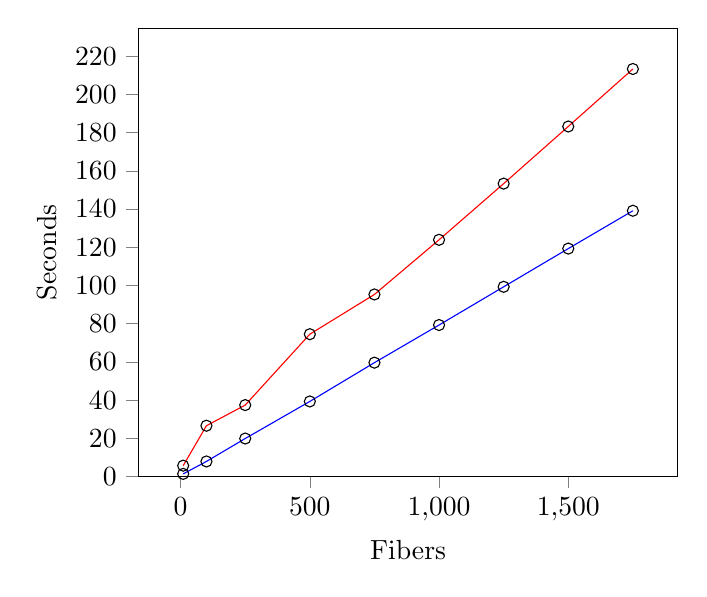
\begin{tikzpicture}
\begin{axis}[%
    ymin=0,
    scatter/classes={%
    a={mark=o,draw=black}},
    xlabel=Fibers,
    ylabel=Seconds,
    ytick={0,20,...,220}, ytick align=outside, ytick pos=left,
    xtick={0,500,...,2000},xtick align=outside, xtick pos=left,
    ]
\addplot[blue, scatter,% KERNEL
    scatter src=explicit symbolic]%
table [meta=label] {
x y label
10 1.4 a
%50 4.1 a
100 7.9 a
250 19.9 a
500 39.3 a
750 59.6 a
1000 79.3 a
1250 99.3 a
1500 119.3  a
1750 139.1 a
};
\addplot[red,scatter,% USER
    scatter src=explicit symbolic]%
table[meta=label] {
x y label
10 5.7 a
%50 10.0 a
100 26.6 a
250 37.4 a
500 74.5 a
750 95.3 a
1000 123.9 a
1250 153.3 a
1500 183.2 a
1750 213.3 a
};
\end{axis}
\end{tikzpicture}
\end{center}

From the plot we can infer a speedup with respect to the userspace implementation ranging from {\tt 4x}, with very few fibers (ten or twenty), to still more than {\tt 1.5x} with more than a thousand of fibers.




\begin{thebibliography}{99}
  \bibitem{fibers}
    Microsoft,
    \path{docs.microsoft.com/en-us/windows/desktop/procthread/fibers},
    2018.

  \bibitem{rbtree}
    Kernel Docs,
    lwn.net/Articles/218239/

\end{thebibliography}

\end{document}
